  % Created 2018-06-21 Thu 12:30
\documentclass[8pt]{beamer}
\usepackage[sc,osf]{mathpazo}   % With old-style figures and real smallcaps.
\linespread{1.025}              % Palatino leads a little more leading
% Euler for math and numbers
\usepackage[euler-digits,small]{eulervm}
%\documentclass[10pt]{llncs}
%\usepackage{llncsdoc}
\usepackage{ifsym}
\usepackage{minted}
\usepackage[utf8]{inputenc}
\usepackage[T1]{fontenc}
\usepackage{fixltx2e}
\usepackage{graphicx}
\usepackage{longtable}
\usepackage{float}
\usepackage{tikz}
\usepackage{tikz-cd}
\usepackage{wrapfig}
\usepackage{rotating}
\usepackage{changepage}
\usepackage[normalem]{ulem}
\usepackage{amsmath}
\usepackage{textcomp}
\usepackage{marvosym}
\usepackage{wasysym}
\usepackage{amssymb}
\usepackage{hyperref}
\usepackage{polynom}
\usepackage{graphicx}
% \usepackage{multirow}
% \usepackage{algorithm2e}
\usepackage{multirow}
\usepackage{latexsym}
\usepackage{physics}
\usepackage{amsmath}
\usepackage{amssymb}
\usepackage{stmaryrd}
% \usepackage{tikz}
\usepackage{multirow}
\usepackage{multicol}
\usepackage{array}
\usepackage{amsthm}
\usepackage{mathtools}
\usepackage{booktabs}
\usepackage{epigraph}
\usepackage{todonotes}
\usepackage{mathtools}

\renewcommand{\mod}[1]{\left( \texttt{mod}~#1 \right)}
\newcommand{\N}{\mathbb N}
\newcommand{\Z}{\mathbb Z}
\newcommand{\Q}{\mathbb Q}
\newcommand{\C}{\mathbb C}
\newcommand{\wtov}{\texttt{word2vec}}
\newcommand{\king}{\texttt{king}}
\newcommand{\man}{\texttt{man}}
\newcommand{\woman}{\texttt{woman}}
\newcommand{\queen}{\texttt{queen}}
\newcommand{\fuzembed}{\texttt{fuzembed}}
\newcommand{\vecembed}{\texttt{vecembed}}
\newcommand{\CORPUS}{\texttt{CORPUS}}
\newcommand{\VOCAB}{\texttt{VOCAB}}
\newcommand{\word}{\texttt{word}}
\newcommand{\fuzzy}{\texttt{fuzzy}}
\newcommand{\fuzz}{\texttt{fuzz}}
\newcommand{\infdiv}{D\infdivx}

\tolerance=1000
\usetheme{Antibes}
\author{Siddharth Bhat}
\date{October 23th, 2021}
\institute{IIIT Hyderabad}
\title{Mathematical structures for word embeddings}
\hypersetup{
  pdfkeywords={},
  pdfsubject={},
  pdfcreator={Emacs 24.5.1 (Org mode 8.2.10)}}
\begin{document}

\maketitle

\begin{frame}[label=sec-1]{What is a word embedding?}
  \pause
\begin{itemize}
  \item Map words to \emph{mathematical objects}.  \pause
  \item Semantic ideas on words $\simeq$ mathematical operations on these objects. \pause
  \item Most common: \emph{vector embeddings} (\texttt{word2vec}) \pause
\end{itemize}
\end{frame}


\begin{frame}{What's \texttt{word2vec}?}
\begin{itemize}
    \item Input: A corpus (sequence of words.). Output: mapping from words to \emph{vectors}.\pause
\end{itemize}
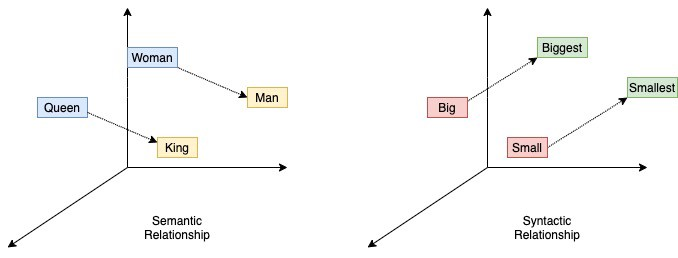
\includegraphics[width=0.8\textwidth]{w2v-linear-relationship.jpeg} \pause
\begin{itemize}
    \item How does one compute such a mapping?  \pause
    \item Distributional Hypothesis: words that occur in the same contexts tend to have similar meanings.\pause
    \item Start with \emph{random vectors}. Make words that occur close by come closer, words that don't occur close by become perpendicular.\pause
\end{itemize}
\end{frame}

\begin{frame}[fragile]{What's \texttt{word2vec}?}
\begin{minted}[fontsize=\small]{python}
def train(corpus: list, DIMSIZE: int):
  """
  train word2vec of dimension DIMSIZE on the given corpus (list of words).
  Eg:train(["the", "man", "was" "tall", "the", "quick", "brown", "fox"], 20)
  """
  vocab = set(corpus); VOCABSIZE = len(vocab)
  # map each unique word to an index for array indexing.
  vocab2ix = dict([(word, ix) for (ix, word) in enumerate(corpus)])
  # +ve and -ve sample vectors.
  # +ve vectors are random initialized, -ve vectors are zero initialized
  poss = np.rand((VOCABSIZE, DIMSIZE)); negs = np.zeros((VOCABSIZE, DIMSIZE))

  for wix in range(len(corpus)): # for every location in the corpus
    w = vocab2ix[corpus[wix]]  # find word at location,
    l = max(wix-WINDOWSIZE, 0); r = min(wix+WINDOWSIZE, len(corpus)-1) # take a window

    for w2ix in range(l, r+1): # word in window
        w2 = vocab2ix[corpus[w2ix]] # prallel.
        learn(l=poss[w], r=negs[w2], target=1.0)

    for _ in range(NNEGSAMPLES): # random words outside window. 
        w2ix = random.randint(0, len(corpus)-1) # random word.
        w2 = vocab2ix[corpus[w2ix]] 
      learn(l=poss[w], r=negs[w2], target=0.0) # perpendicular
  return { v: poss[vocab2ix[v]] for v in vocab } 
\end{minted}
\end{frame}

\begin{frame}[fragile]{What's \texttt{word2vec}?}
\begin{minted}[fontsize=\small]{python}
def learn(l: np.array, r:np.array, target: float):
  """
  gradient descent on
  loss = (target - dot(l, r))^2 where l = larr[lix]; r = rarr[rix]
  """
  dot = np.dot(l, r); grad_loss = 2 * (target - out)
  #dloss/dl = 2 * (target - dot(l, r)) r
  #dloss/dr = 2 * (target - dot(l, r)) l
  lgrad =  EPSILON * grad_loss * r; rgrad =  EPSILON * grad_loss * l
  # l -= eps * dloss/dl; r -= eps * dloss/dr
  l += EPSILON * grad_loss * r;
  r += EPSILON * grad_loss * l

def train(corpus: list, DIMSIZE: int):
    for w2ix in range(l, r+1): # positive samples, parallell
        w2 = vocab2ix[corpus[w2ix]] # word in window
        learn(l=poss[w], r=negs[w2], target=1.0)
    for _ in range(NNEGSAMPLES): # negative samples: perpendicular. 
        w2ix = random.randint(0, len(corpus)-1) # random word outside window.
        learn(l=poss[w], r=negs[w2], target=0.0) # perpendicular
\end{minted}
\end{frame}



% \begin{frame}{How do we use \texttt{word2vec}?}
%     \item Dot products capture similarity. \pause
%     \item nope! \emph{cosine similarity} captures similarity: $v \cdot w / |v| |w|$. \pause
%     \item Vector space structure captures analogy: $\king - \man + \woman = \queen$. [Analogy] \pause
%     \item nope! $normalize(\hat \king - \hat \man + \hat \woman) = \hat \queen$ \pause
%     \item \wtov "vectors" are always normalized! \pause
%     \item Cannot add, subtract, scale. So in what sense is the embedding "vectorial"? \pause
%     \item In the sense that we have "vectors" --- elements of the space $[-1, 1]^N$ with a normalization condition $(\sum_i x_i^2 = 1)$. \pause
%     \item Can we ascribe a \emph{different} meaning to these "vectors"?
% \end{itemize}
% \end{frame}

\begin{frame}{Part I: What's a philosopher to do?}
\begin{itemize}
    \item Montague semantics: The \emph{meaning} of a word is the \emph{set} of possible worlds where the meaning holds true. \pause
    \item A mathematical analogy: The \emph{meaning} of an expression $\forall x \in \Z, x \leq 2$ is... \pause
    \item  the \emph{set} of possible values where the meaning holds true: $(-\infty, 2] = \{  x \in \Z : x \leq 2 \}$. \pause
    \item Meaning $\simeq$ subsets. Is  \wtov~ subsets?  \pause Yes, \emph{fuzzy sets}. \pause
    \item Set: binary membership. ($1 \in_? \{1, 2\} = T$, $3 \not \in_? \{1, 2\} = F$). \pause
    \item Fuzzy set: probabilistic membership. ($1 \in_{fuz} F = 0.1$, $2 \in_{fuz} F = 0.5$).
    \item Formally:  $A \equiv \{ (x, \mu_A(x)), x \}$. $x$ is
      an element of set $A$ with a probability $\mu_A(x)$ such that $0 \leq \mu_A(x) \leq 1$
\end{itemize}
\end{frame}

\begin{frame}{The hidden sets in \texttt{word2vec}}
\begin{itemize}
  \item Given the set of vectors, normalize the $i$th component of the vector across \emph{all vectors}. \pause
  \item $\fuzembed_{\word}[i] \equiv e^{\vecembed_{\word}[i]} / \sum_{w \in \CORPUS} e^{\vecembed_w[i]}$. \pause
  \item Fuzzy set embedding from \texttt{word2vec}~embeddings. \pause
  \item The projection of $\vec v$ on a dimension $i$ normalized  is to be interpreted as
  if this dimension $i$ were a property, what is probability that $v$ would possess that property?
\end{itemize}
\end{frame}

\begin{frame}{What does this buy us anyway? (Set operations)}
\begin{align*} &(A \cap B)[i] \equiv  A[i] \times B[i] \quad \text{(set intersection)} \\
&(A \cup B)[i] \equiv  A[i] + B[i]  - A[i] \times
B[i] \, \text{(set union)}\\ &(A \sqcup B)[i] \equiv  \max(1, \min(0, A[i] +
B[i])) \, \text{(disjoint union)}\\ &(\lnot A)[i] \equiv 1 - A[i] \quad
\text{(complement)}\\ &(A \setminus B)[i] \equiv A[i]  - \min(A[i], B[i]) \quad
\text{(set difference)} \\ &(A \subseteq B) \equiv \forall x \in \Omega:
\mu_A(x) \leq \mu_B(x) \, \text{(set inclusion)}\\ &|A| \equiv \sum_{i \in \Omega} \mu_A (i) \quad \text{(cardinality)} \\
\end{align*}
\end{frame}

\begin{frame}{What does this buy us anyway? (Set intersection)}

% \begin{equation*}
%    H(S, T) \equiv \sum_i H(X^S_i) + KL(X^S_i, X^T_i)
% \end{equation*}

     \begin{tabular}{l l l l l}
         $\hat N$    & $\hat M$  & $\hat G$  & $\hat N \cap \hat M$  & $\hat N \cap \hat G$      \\
         nobility    & metal     & bad       & fusible               & good                      \\
         isotope     & fusible   & manners   & unreactive            & dharma                    \\
         fujwara     & ductility & happiness & metalloids            & morals                    \\
         feudal      & with      & evil      & ductility             & virtue                    \\
         clan        & alnico    & excellent & heavy                 & righteous             \\ \midrule
         $\vec N$    & $\vec M$  & $\vec G$  & $\vec N + \vec M$     & $\vec N + \vec G$         \\
         noblest     & trivalent & bad       & fusible               & gracious                  \\
         auctoritas  & carbides  & natured   & metals                & virtuous                  \\
         abies       & metallic  & humoured  & sulfides              & believeth                 \\
         eightfold   & corrodes  & selfless  & finntroll             & savages                   \\
         vojt        & alloying  & gracious  & rhodium               & hedonist
   \end{tabular}

\begin{itemize}
\item Polysemy of the word \texttt{noble}, in the context of the words \texttt{good} and \texttt{metal}.
\item \texttt{noble} is represented by $N$, \texttt{metal} by $M$ and \texttt{good} by $G$.
\item We also provide the word2vec analogues of the same, under $\vec N$, $\vec M$, and $\vec G$.
\item See that \texttt{word2vec} has no analogue for set-intersection. We use the closest possible analogue (addition), which performs worse semantically.
\end{itemize}

\end{frame}

\begin{frame}{Crash course on entropy}
\begin{itemize}
\item Given a probability $p \in [0, 1]$, define the \emph{surprisal} to be $- \log_2 p$. \pause
\item  If $p = 1$, and the event happens, then we are never ($- \log_2 1 = 0$) surprised. \pause
\item  If $p = 0$, and the event happens, then we are terrifically ($- \log_2 0 = - (-\infty) = +\infty)$ surprised. \pause
\item  If $p = 1/2$, and the event happens, then we are terrifically ($- \log_2 1/2 = - (-1) = +1)$ surprised. \pause
\item Given a distribution $P: X \to [0, 1]$, the entropy of $P$ is the \emph{average surprise}, given by $\sum_{x \in X} P(x) \cdot - \log P(x)$.  
\end{itemize}
\end{frame}

\begin{frame}{What does this buy us anyway? (Entropy)}
Fuzzy entropy is a measure of the uncertainty of the elements belonging to the set. \pause

\begin{align*} H(A) &\equiv \sum_i H(X^A_i) \\ &\equiv \sum_i
-p_i^A \ln p_i^A - (1 - p_i^A) \ln (1 - p_i^A) \\ &\equiv  \sum_i -A[i] \ln
A[i] - (1 - A[i]) \ln (1 - A[i])
\end{align*}


\begin{tabular}{l r | l r | l r | l r | l r}
and   & the   &   in    &   one         &   which     &   to          &   however &   \emph{two}  &   for     &   \emph{eight}  \\
this    & of    &   of      &   in          &   the       &   \emph{zero} &   to    &   is          &   a     &   for \\
as      & and   &   only  &   a           &   also      &   \emph{nine} &   it    &   as          &   but     &   \emph{s}
\end{tabular}

\begin{itemize}
\item Function words are words which are largely syntactic rather than semantic.
\item On the left: Top 15 words with highest entropy with frequency $\geq 100$. (note that all of them are function words).
\item On the right: Top 15 words with the highest frequency.
\item Non-function words are emphasized for comparison.
\end{itemize}
\end{frame}

\begin{frame}{What does this buy us anyway? (KL divergence)}
  \begin{itemize}
    \item K-L (Kullback Leibler) divergence is an asymmetric measure of similarity.
    \item Given data d which follows distribution P, the extra bits need to store
      it under the false assumption that the data d follows distribution Q is the K-L divergence
      between the distributions P and Q.
    \end{itemize}
  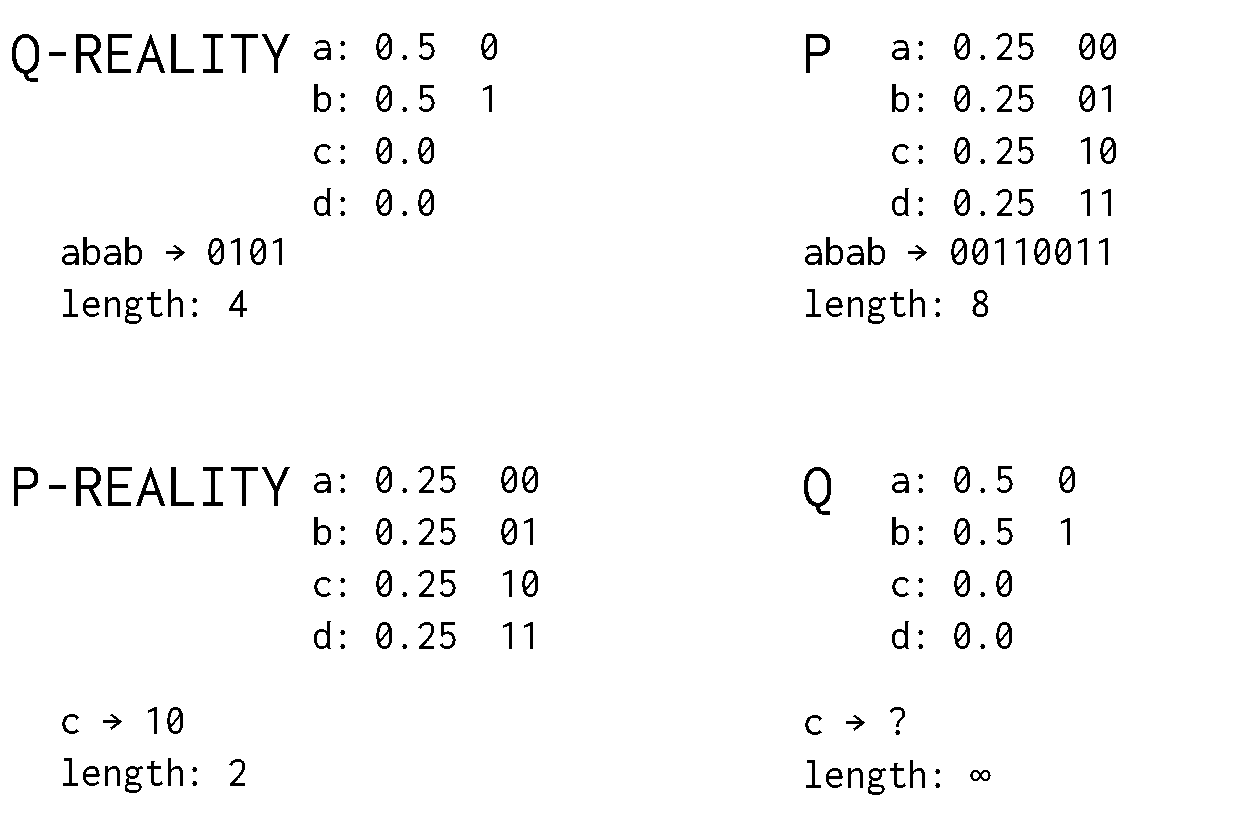
\includegraphics[width=0.8\textwidth]{./kl-divergence-asymmetry.pdf}
\end{frame}

\begin{frame}{What does this buy us anyway? (KL divergence)}
\begin{itemize}
 \item K-L (Kullback Leibler) divergence is an asymmetric measure of similarity.
 \item Given data d which follows distribution P, the extra bits need to store
    it under the false assumption that the data d follows distribution Q is the K-L divergence
    between the distributions P and Q.
\item Let $P$ be the distribution that assigns $0.25$ probability to $a, b, c, d$. Since all are equiprobable, we use $2$ bits per character.
\item Let $Q$ be the distribution that assigns $0.5$ probability to $a, b$ and $0$ probability to $c, d$. We use $1$ bit to represent if we are storing $a$ or $b$.
\item If the real distribution is $Q$ and we store data using $P$, then we really need only $\{a, b\}$, but we are trying to store $\{a, b, c, d\}$. $P$(false assumption) needs
  twice as many bits as $Q$(true distribution) to store the message $c$.
\item If the real distribution is $P$ and we store data using $Q$, then we really need $\{a, b, c, d\}$, but we \emph{can only store} $\{a, b\}$. $Q$(false assumption)
  need \emph{infinitely} more bits to store the message $c$ than $P$ (true distribution).
\end{itemize}
\end{frame}

\begin{frame}{What does this buy us anyway? (KL divergence)}


\begin{equation*}
     KL(S, T) \equiv \sum_i KL(X^S_i, X^T_i) =  \sum_i p^S_i \log \left( p^S_i / p^T_i \right)
\end{equation*}


\begin{tabular}{clr}
    \multirow{2}{*}{Example 1} & $KL(ganges, delta)$ & $6.3105$  \\
                               & $KL(delta, ganges)$ & $6.3040$  \\
    \multirow{2}{*}{Example 2} & $KL(north \cap korea, china)$ & $1.02923$ \\
                               & $KL(china, north \cap korea)$ & $10.60665$
\end{tabular}
% Examples of KL-divergence as an asymmetric measure of similarity. Lower is closer.
% We see here that the evaluation of North Korea as a concept being closer to China than vice versa can be observed by the use of
% K-L Divergence.

\begin{itemize}
\item  K-L divergence shows the relation
between two words.
\item Can also consider phrases when composed using feature intersection as in the case of
north korea.
\item We demonstrate human annotator judgement of the distance between China
and North Korea, where human annotators considered ``North Korea'' to be very similar to
``China'', while the reverse relationship was rated as significantly less strong (``China'' is not
very similar to ``North Korea'')
\end{itemize}
\end{frame}

\begin{frame}{What does this buy us anyway? (Cross entropy)}

\begin{itemize}
\item cross-entropy of two distributions $P$ and $Q$ is the sum of the entropy of
$P$ and the K-L divergence between $P$ and $Q$. 
\item captures both the \emph{uncertainty in $P$}, as well as the distance from $P$ to $Q$.
\item Gives information theoretic difference between the concepts
of $P$ and $Q$.
\end{itemize}
\end{frame}

\begin{frame}{What does this buy us anyway? (Analogy)}

\begin{equation*}
\begin{split}
    &a : b :: x : y_? \\
    &y_? = b - a + x \implies y_? = (b + x) - a \\
    &y = (b \sqcup x) \setminus a \quad \text{(Set-theoretic interpretation)}
\end{split}
\end{equation*}


\begin{itemize}
\item given a pairing $(a : b)$, and a prior $x$, we are asked to compute an unknown
word $y_?$ such that  $a:b::x:y_?$
\item In the vector space model, analogy is computed based on vector distances. But this is semantically incoherent, as we must then re-normalize vectors.
\item 
\end{itemize}
\begin{tabular}{ccc|c|c}
    \bf Word 1  & \bf Word 2    & \bf Word 3    & \bf word2vec  & \bf Our representation    \\ \hline
    bacteria    & tuberculosis  & virus         & polio         & hiv                       \\
    cold        & freezing      & hot           & evaporates    & boiling                   \\
    ds          & nintendo      & dreamcast     & playstation   & sega                      \\
    pool        & billiards     & karate        & taekwondo     & judo                      \\
\end{tabular}
\begin{itemize}
  \item Examples of analogy compared to the analogy in word2vec. We see here that the comparisons constructed by feature representations are similar to those given by the standard word vectors.
\end{itemize}
\end{frame}

\begin{frame}{Evaluation: Similarity}

   \begin{tabular}{c|c|cc}
        \multirow{2}{*}{\bf Dims.}   & \multirow{2}{*}{\bf word2vec} & \multicolumn{2}{c}{\bf Our Representation} \\ \cline{3-4}
                            &                               & K-L Divergence & Cross-Entropy \\\hline
        20  &   0.2478   & 0.2690 & \bf 0.2744    \\
        50  &   0.2916   & 0.2966 & \bf 0.2981    \\
        100 &   0.2960   & 0.3124 & \bf 0.3206    \\
        200 &   0.3259   & 0.3253 & \bf 0.3298
    \end{tabular}

  \begin{itemize}
    \item Similarity scores on the SimLex-999 dataset for various dimension sizes (Dims.).
  \end{itemize}
\end{frame}

\begin{frame}{Evaluation: Analogy}

\scalebox{0.5}{
    \begin{tabular}{ll|rr|rr}
        \multicolumn{2}{l|}{\bf\multirow{2}{*}{Category}}& \multicolumn{2}{c|}{\bf word2vec} & \multicolumn{2}{c}{\bf Our representation}   \\ \cline{3-6}
        \multicolumn{2}{l|}{}                           & 50        & 100       & 50        & 100               \\\hline
        \multicolumn{2}{l|}{Capital Common Countries}   & 21.94     & 37.55     & \bf 39.13 & \bf 47.23         \\
        \multicolumn{2}{l|}{Capital World}              & 13.02     & 20.10     & \bf 27.30 & \bf 26.54         \\
        \multicolumn{2}{l|}{Currency}                   & 12.24     & 18.60     & \bf 25.27 & \bf 24.90         \\
        \multicolumn{2}{l|}{City-State}                 & 10.38     & 16.70     & \bf 23.24 & \bf 23.51         \\
        \multicolumn{2}{l|}{Family}                     & 10.61     & 17.34     & \bf 23.67 & \bf 23.88         \\ \hline
        \multirow{3}{*}{Adjective-Adverb}   & Syntactic & 4.74      & 3.23      & \bf 7.26  & \bf 3.83          \\
                                            & Semantic  & 10.61     & 17.34     & \bf 23.67 & \bf 23.88         \\
                                            & Overall   & 9.92      & 15.68     & \bf 21.73 & \bf 21.52         \\ \hline
        \multirow{3}{*}{Opposite}           & Syntactic & 4.06      & 3.66      & \bf 7.61  & \bf 4.92          \\
                                            & Semantic  & 10.61     & 17.34     & \bf 23.67 & \bf 23.88         \\
                                            & Overall   & 9.36      & 14.73     & \bf 20.60 & \bf 20.26         \\ \hline
        \multirow{3}{*}{Comparative}        & Syntactic & 8.86      & 12.63     & \bf 16.88 & \bf 15.39         \\
                                            & Semantic  & 10.61     & 17.34     & \bf 23.67 & \bf 23.88         \\
                                            & Overall   & 10.10     & 15.96     & \bf 21.67 & \bf 21.39         \\ \hline
        \multirow{3}{*}{Superlative}        & Syntactic & 7.59      & 11.30     & \bf 14.32 & \bf 13.36         \\
                                            & Semantic  & 10.61     & 17.34     & \bf 23.67 & \bf 23.88         \\
                                            & Overall   & 9.54      & 15.20     & \bf 20.35 & \bf 20.15         \\ \hline
        \multirow{3}{*}{Present-Participle} & Syntactic & 7.51      & 10.96     & \bf 14.31 & \bf 13.14         \\
                                            & Semantic  & 10.61     & 17.34     & \bf 23.67 & \bf 23.88         \\
                                            & Overall   & 9.34      & 14.73     & \bf 19.84 & \bf 19.49         \\ \hline
        \multirow{3}{*}{Nationality}        & Syntactic & 12.51     & 19.07     & \bf 21.64 & \bf 21.96          \\
                                            & Semantic  & 10.61     & 17.34     & \bf 23.67 & \bf 23.88         \\
                                            & Overall   & 11.51     & 18.16     & \bf 22.71 & \bf 22.97         \\ \hline
        \multirow{3}{*}{Past Tense}         & Syntactic & 11.65     & 17.09     & \bf 20.43 & \bf 19.76         \\
                                            & Semantic  & 10.61     & 17.34     & \bf 23.67 & \bf 23.88         \\
                                            & Overall   & 11.16     & 17.21     & \bf 21.96 & \bf 27.72         \\ \hline
        \multirow{3}{*}{Plural}             & Syntactic & 11.76     & 17.23     & \bf 20.53 & \bf 19.89         \\
                                            & Semantic  & 10.61     & 17.34     & \bf 23.67 & \bf 23.88         \\
                                            & Overall   & 11.26     & 17.28     & \bf 21.90 & \bf 21.64         \\ \hline
        \multirow{3}{*}{Plural Verbs}       & Syntactic & 11.36     & 16.60     & \bf 19.88 & \bf 19.46         \\
                                            & Semantic  & 10.61     & 17.34     & \bf 23.67 & \bf 23.88         \\
                                            & Overall   & 11.05     & 16.91     & \bf 21.46 & \bf 21.30         \\ \hline
    \end{tabular}
}
\begin{itemize}
\item Comparison of Analogies between word2vec and our representation for 50 and 100 dimensions (Dims.).
\item Outperform word2vec on every single metric.
\end{itemize}
\end{frame}


\begin{frame}{Evaluation: Function word detection}
    \begin{tabular}{c|cc}
        top $n$ words & \bf word2vec & \bf Our Representation  \\ \hline
        15  & 10 & \bf 15 \\
        30  & 21 & \bf 30 \\
        50  & 39 & \bf 47  \\
    \end{tabular}

\begin{itemize}
\item Function word detection using entropy (in our representation) and by frequency in word2vec.
\item We see that we consistently detect more function words than word2vec, based on the 176 function word list (Making and Using Word Lists for Language Learning and Teaching).
\item The metric is \emph{number of words}, i.e. the number of words chosen by frequency for word2vec and entropy for our representation.
\item We detect more function words than the baseline frequency based methods. 
\end{itemize}
\end{frame}


\begin{frame}{Evaluation: Compositionality detection}
    \begin{tabular}{c|c|cc}
        \bf Dims.               & \bf Metric& \bf word2vec  & \bf Our Representation    \\ \hline
        \multirow{2}{*}{50}     & Spearman  & 0.3946    & \bf 0.4117            \\
                                & Pearson   & 0.4058    & \bf 0.4081            \\ \hline
        \multirow{2}{*}{100}    & Spearman  & 0.4646    & \bf 0.4912            \\
                                & Pearson   & 0.4457    & \bf 0.4803            \\ \hline
        \multirow{2}{*}{200}    & Spearman  & 0.4479    & \bf 0.4549            \\
                                & Pearson   & \bf 0.4163& 0.4091                \\
    \end{tabular}
\begin{itemize}
  \item Predict whether two words combine to create a phrase or not (eg. monkey business, silver bullet)
  \item We decide that a phrase $w_1 w_2$ is a phrase if $|KL(w_1, w_2) - KL(w_2, w_1)|$ is large, as this implies information asymmetry.
  \item We see that almost across the board, we perform better.
\end{itemize}
\end{frame}

\begin{frame}{Conclusion}
  \begin{itemize}
    \item \texttt{word2vec} is performant but poorly understood.
    \item We extract fuzzy set embeddings from \texttt{word2vec}, giving richer, understandable variants of vector-based operations!
    \item TL;DR: Mathematical modelling (fuzzy sets) is useful to extend empirical results (\texttt{word2vec})!
    \item \url{https://www.aclweb.org/anthology/2020.repl4nlp-1.4/}
    \item Collaborators: Alok Debnath, Souvik Banerjee.
    \item Advisors: Dr. Kannan Srinathan, Dr Manish Shrivastava.
  \end{itemize}
  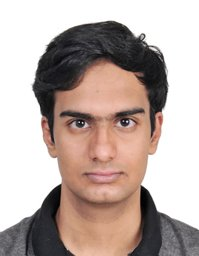
\includegraphics[width=0.2\textwidth]{./alok.jpeg}
  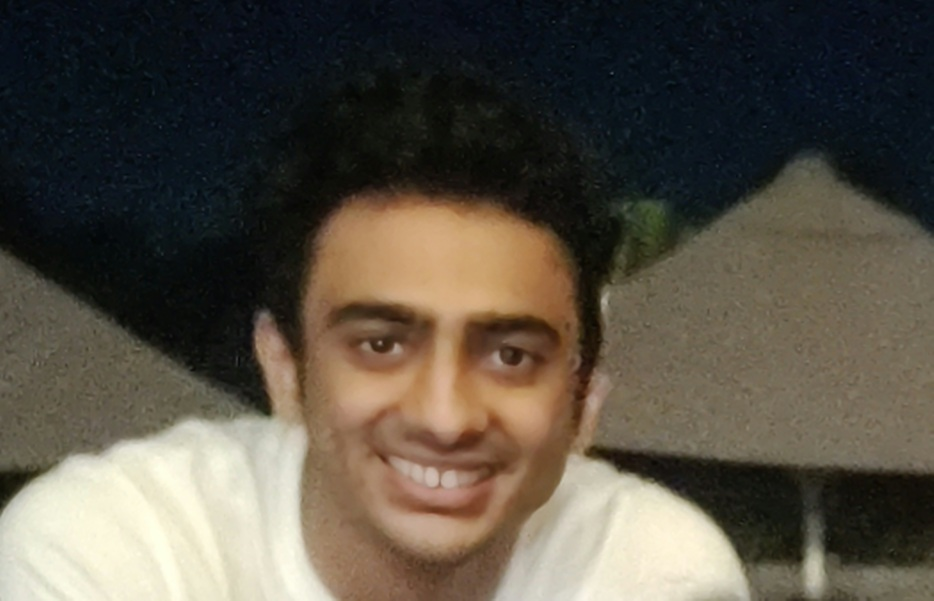
\includegraphics[width=0.3\textwidth]{./souvik.jpg}
\end{frame}


\begin{frame}{Extensions}
  \begin{itemize}
    \item The only thing we need to train \texttt{word2vec} is a dot-product. \pause
    \item Can we generalize? \texttt{word2vec} consider \emph{directions}, which are 1D subspaces. \pause
    \item We should generalize! Use nD subspaces. \pause
    \item The collection of all nD subspaces of a vector space is known as the \emph{Grassmanian}. \pause
  \end{itemize}
\end{frame}


\begin{frame}{Training on the grassmanian}
  \begin{itemize}
    \item The collection of all nD subspaces of a vector space is known as the \emph{Grassmanian}. \pause
    \item What is the analogue of the dot-product? It is an operation known as \emph{Angle between flats}.
  \end{itemize}
  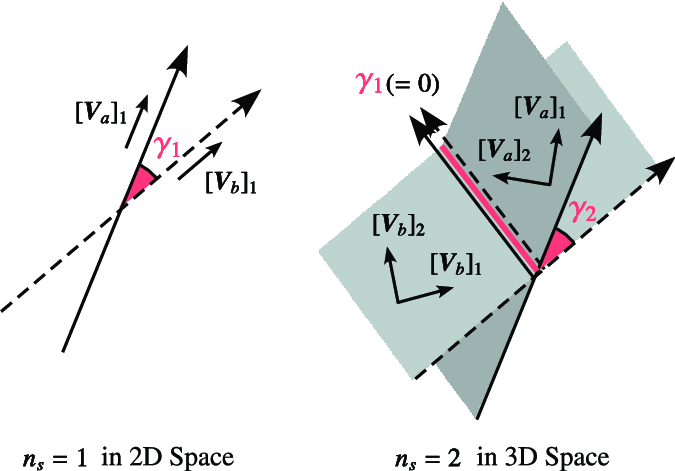
\includegraphics[width=0.5\textwidth]{./angles-between-flats.png}
  \begin{itemize}
    \item How does one take gradients on the Grassmanian?
  \end{itemize}
\end{frame}

\begin{frame}{Training on the grassmanian(2)}
  \begin{itemize}
    \item Space $\equiv$ Grassmanian (orthonormal vectors representing subspace) $\simeq$ orthogonal matrix.
    \item Random Initialization $\equiv$ (1) Random matrix, (2) $Q$ part of $QR$ decomposition.
    \item Dot product $\equiv$ Angle between subspaces
    \item Gradient Descent $\equiv$ (1) Regular gradient descent, (2) retraction: $Q$ part of $QR$ decomposition 
  \end{itemize}
\end{frame}

\begin{frame}{Results for training on the grassmanian [Sovik Banerjee's research]}

\begin{itemize}
\item We evaluate the quality of our document embed-dings with the 20newsgroups topic classification.
\item k-NN algorithm on Grassmannian manifold is performed by replacing
  the euclidean metric with grassmanian-compatible metric
\end{itemize}

\begin{tabular}{lll} \hline
Embedding & F1-Macro & F1-Micro\\ \hline
Avg. W2V & 0.630 & 0.631\\ \hline
SIF & 0.552 & 0.549 \\ \hline
Doc2Vec & 0.648 & 0.645 \\ \hline
JoSE & 0.703 & 0.707 \\ \hline
Grassmannian & \textbf{0.749} & \textbf{0.752}\\
\hline
\end{tabular}
% \caption{Results of the $k$-NN ($k$=3) classification task with 20 Newsgroups dataset}
% \label{tab:20news-classification-results}
% \end{table}

\begin{itemize}
  \item we performed sentiment analysis on the imdb movie reveiew dataset using kernel SVM.
  \item We see that our model slightly outperforms the other embeddings model.
\end{itemize}

\begin{tabular}{lll} \hline
Embedding & Accuracy\\ \hline
Avg. W2V & 88.02\\ \hline
SIF & 85.32 \\ \hline
Doc2Vec & 88.52 \\ \hline
JoSE &  87.95\\ \hline
Grassmannian & \textbf{88.90}\\
\hline
\end{tabular}
% \caption{Sentiment analysis accuracy results}
% \label{tab:imdb-sentiment-results}
% \end{table}

\end{frame}

\begin{frame}{Abstract interpretation}
\begin{itemize}
    \item $\alpha: (C, \leq) \to (A, \sqsubset)$: monotone Abstraction from the Concrete to the Abstract.
    \item $\gamma: (A, \sqsubset) \to (C, \sqsubset)$: monotone Concretization from Abstract to the Concrete. ($\gamma$ for Galois)
    \item $c \leq \gamma(\alpha(c))$: Abstraction can lose information
    \item $a = \alpha(\gamma(c))$: Concretization is faithful: abstract objects are well represented by concrete objects.
\end{itemize}

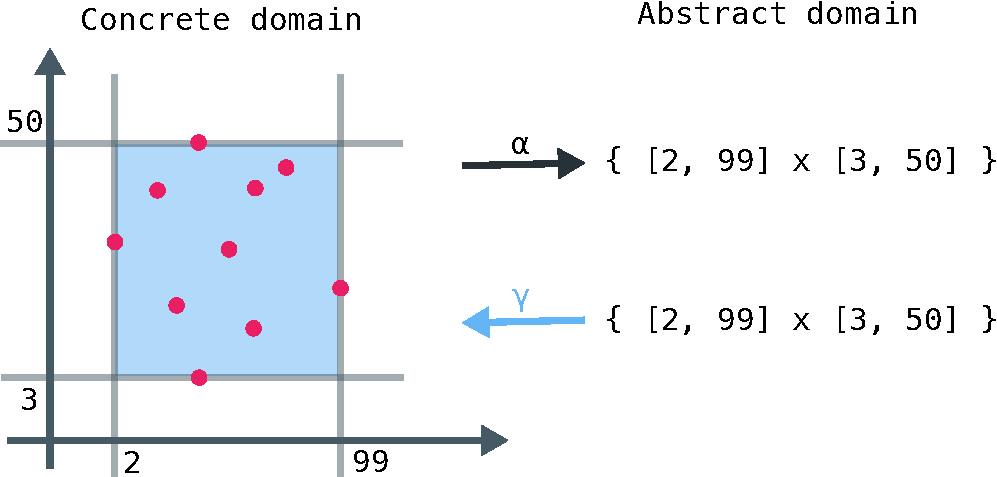
\includegraphics[width=0.8 \textwidth]{../alpha-gamma-intervals.pdf}
\end{frame}

\begin{frame}{Montague semantics via abstract interpretation}
\begin{itemize}
  \item A common abstraction is given by special types of subsets (eg. intervals)
  \item These are useful since they form a lattice.
  \item Try to extract these out from \texttt{word2vec}
\end{itemize}
\end{frame}


\end{document}

